\documentclass{article}
\usepackage[utf8]{inputenc}
\usepackage[T1]{fontenc}
\usepackage{polski}
\usepackage{indentfirst}
\usepackage{lastpage}
\usepackage{graphicx} 
\usepackage{sidecap}
\usepackage{wrapfig}
\usepackage{subfig}

\usepackage{caption}
\captionsetup[figure]{name={Obrazek}}

\usepackage{fancyhdr}
\pagestyle{fancy}
\fancyhf{}
\rhead{Franciszek Wysocki, Bartosz Zdybel}
\rfoot{Strona \thepage \hspace{1pt} z \pageref{LastPage}}
\lhead{Spis treści}
\title{Sprawozdanie końcowe dla projektu w javie pt. \\ ,,BattleZone''}
\author{}
\date{}

\begin{document}
\maketitle

\begin{flushright}
\par ...
\vfill
\par
Wykonali: Franciszek Wysocki, Bartosz Zdybel

Sprawdzający: mgr inż. Paweł Zawadzki

Data: 01.06.2020
\end{flushright}

\thispagestyle{empty}
\newpage
\begin{frame}{}
    \tableofcontents
\end{frame}
\newpage
\lhead{Cel projektu}
\section{Cel projektu}

Celem projektu było stworzenie programu w języku Java, który będzie posiadał graficzny interfejs użytkownika (Grapical User Interface, GUI) i  umożliwi rywalizację dwóm graczom poprzez poruszanie się czołgami i strzelanie do komórek.
Głównymi założeniami gry, którą nazwaliśmy ,,BattleZone'' są:
\begin{itemize}
\item wczytywanie danych z pliku wejściowego o rozszerzeniu txt
\item umożliwienie dwóm graczom poruszania się czołgami 
\item stworzenie planszy z komórkami
\item zmniejszanie komórek co określony czas podany przez użytkownika
\item stworzenie komórek dzieci, które będą powstawać według sąsiedztwa Moore'a
\item stworzenie pocisków i ich przyspieszanie co określony czas
\item stworzenie komórki armagedon, której zestrzelenie automatycznie kończy grę
\item zapisanie stanu końcowego gry do pliku graficznego o rozszerzeniu png
\end{itemize}

\section{Struktura projektu}
Główną klasą znajdującą się w naszym projekcie jest klasa Game, która dziedziczy po klasie JFrame. Klasa ta zawiera metodę main.
W programie również zostały wyróżnione poniższe klasy:
\begin{itemize}
\item Cell - klasa reprezentująca komórkę
\item Cells - klasa obsługująca i przechowująca listę komórek
\item SpriteCells - klasa odpowiedzialna obsługę grafikę komórek
\item GamePanel - główny panel gry
\item MenuPanel - panel startowy
\item Results - klasa wyliczeniowa przechowująca możliwe zakończenia programu
\item ResultsPanel - panel końcowy z wyświetleniem zwycięzcy oraz możliwością zapisu do pliku graficznego
\item Bullet - klasa obsługująca pociski
\item Player - klasa abstrakcyjna reprezentująca gracza
\item LeftPlayer/RightPlayer - klasa obsługująca lewego i prawego gracza
\item InputFileReadeer - klasa odpowiedzialna za wczytanie danych z pliku konfiguracyjnego
\item KeyListener - klasa odpowiedzialna za ,,nasłuchiwanie" klawiszy 
\item Sounds - klasa odpowiedzialna za dźwięk

\end{itemize}
Na poniższym zdjęciu (Obrazek 1) przedstawiona jest struktura projektu:

\begin{figure} [hbt!]
    \centering
    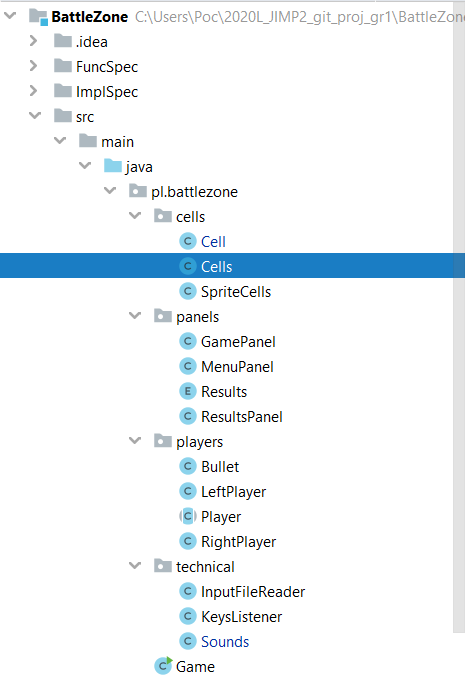
\includegraphics[width=8cm]{Struktura_projektu.png}
   \captionof{figure}{}
\end{figure}


Zaimplementowaliśmy również 39 testów, które sprawdzają poprawność wybranych metod. Strukturę klas zawierającą testy znajduje się na obrazku poniżej (Obrazek 2):

\begin{figure} [hbt!]
    \centering
    \includegraphics[width=7cm]{Struktura_testow.png}
    \captionof{figure}{}
\end{figure}

\lhead{Struktura projektu}

\section{Różnice miedzy specyfikacjami}
Program w większości powstał z głównym planem opisanym szczegółowo w specyfikacji implementacyjnej oraz specyfikacji funkcjonalnej.
Niemniej jednak dokonaliśmy kilku zmian.
\newline Pierwszą zmianą jest modyfikacja pliku wejściowego, który różni się formą wprowadzanych danych. W specyfikacji funkcjonalnej założyliśmy, że w pliku wielkość planszy podajemy w następujący sposób:
20X20, zmodyfikowaliśmy to do takiej postaci:
\newline A=500
\newline B=500
\newline Było to spowodowane łatwiejszym sprawdzeniem błędów wprowadzonych przez użytkownika oraz chęcią uspójnienia danych w pliku, dzięki czemu mogliśmy tylko raz napisać metodę odczytującą i wykorzystać ją dla każdej zmiennej (zgodnie z zasadą DRY).
Drugą modyfikacją było usunięcie z pliku ostatniej zmniennej - M (maksymalna ilość punktów przewidziana na daną rozgrywkę), aby było to zgodne z wymaganiami i aby użytkownik mógł dostosowywać tę wielkość bez konieczności wchodzenia w plik konfiguracyjny.
\newline Ponadto zostały dodane klasy: 
\begin{itemize}
\item Sound (klasa odpowiedzialna za dźwięk) 
\item ResultsPanel (klasa odpowiedzialna za wyświetlenie wyniku i możliwość zapisu końcowego stanu gry do pliku tekstowego)
\item Results (typ wyliczeniowy (enum) przechowujący możliwe zakończenia gry)
\item SpriteCells (klasa zajmującej się obsługiwaniem graficznym komórek)
\end{itemize}

Stworzyliśmy również nowy algorytm, który tworzy według sąsiedztwa Moor'a komórki dzieci wokół komórki rodzica. Algorytm sprawdza po kolei czy miejsca wokół komórek rodzica są wolne miejsca oraz czy wstawiona komórka-dziecko zmieści się w planszy i jeśli tak to tworzy tę komórkę.

\lhead{Różnice między specyfikacjami}
\section{Testowanie}
Testy jednostkowe można np. uruchomić zarówno za pomocą środowiska Intellij lub Mavena.
Efekt działania zaprezentowany na zdjęciu poniżej (Obrazek 3):
\begin{figure} [hbt!]
    \centering
    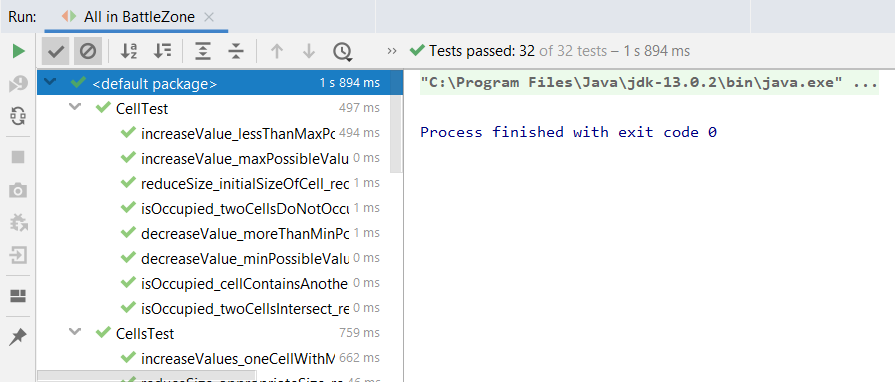
\includegraphics[width=12cm]{Uruchominie_testow.png}
   \captionof{figure}{}
\end{figure}

W przypadku wprowadzenia modyfikacji do jednego testu, by działał niepoprawnie otrzymujemy informację o błędzie (Obrazek 4):
\lhead{Testowanie}
\begin{figure} [hbt!]
    \centering
    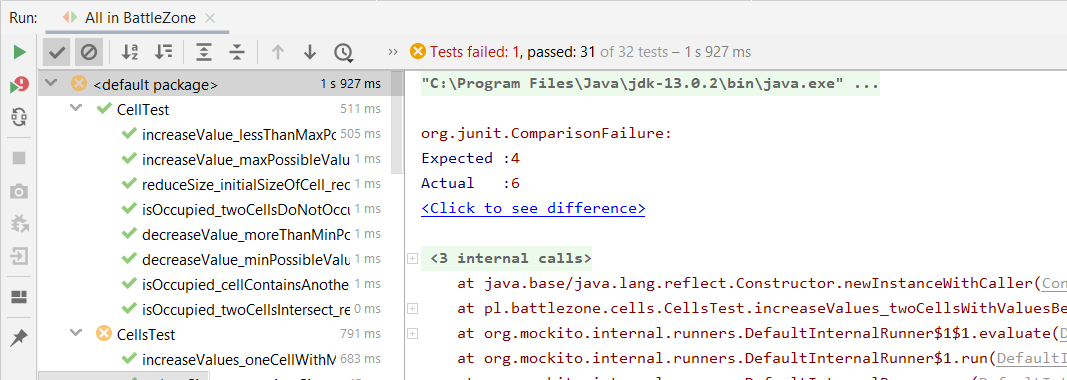
\includegraphics[width=12cm]{bledne_testy.png}
   \captionof{figure}{}
\end{figure}

Testy korzystają z bibliotek: JUnit4, AssertJ oraz Mockito, a ich szkielet jest zgodny z schematem given/when/then. Nazwy testów są wzorowane konwencją ,,nazwaMetody\_podaneDane\_oczekiwanyResultat()''. 
Testy były pisane równolegle do powstawania kodu.

Poza testami jednostkowymi program został przetestowany także manualnie, a ewentualne poprawki były korygowane na bieżąco. Działanie to pozwoliło zabezpieczyć program przed ewentualnymi błędami użytkownika o czym więcej w sekcji ,,Reakcja na błędy''.
\newpage

\section{Reakcje na błędy}
W projekcie zostały wyróżnione 2 rodzaje błędów: zwykłe i krytyczne. Te pierwsze pozwalają na korektę ze strony użytkownika, te drugie natomiast kończą działanie programu.

\lhead{Reakcje na błędy}
\subsection{Błędy zwykłe}

W przypadku gdy użytkownik chce wprowadzić plik z błędnym formatem, program mu na to nie pozwoli i wyświetli stosowny komunikat (Obrazek 5):
\begin{figure} [hbt!]
    \centering
    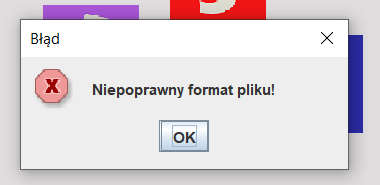
\includegraphics[width=7cm]{blad_1.png}
    \captionof{figure}{}
\end{figure}
\newline
Program zadziała podobnie w odpowiedzi na:
\newline Pozostawienie pustych miejsc w nazwie gracza, maksymalnej liczbie punktów i czasie rozgrywki - pola te zostają one wypełnione włówczas wartościami domyślnymi.
\newline
Błędnie wprowadzone dane: (Obrazek 6 i 7):
\begin{figure} [hbt!]
    \centering
    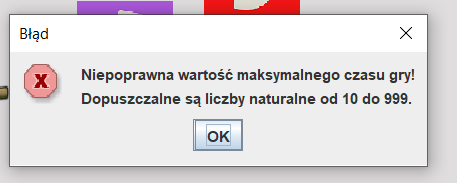
\includegraphics[width=7cm]{blad_2.png}
    \captionof{figure}{}
\end{figure}

\begin{figure} [hbt!]
    \centering
    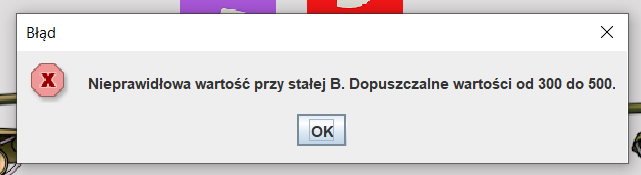
\includegraphics[width=9cm]{blad_3.png}
    \captionof{figure}{}
\end{figure}

Przypadkowe zamknięcięcie programu - wyświetlenie potwierdzenie (Obrazek 8):
\begin{figure} [hbt!]
    \centering
    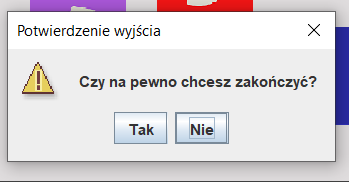
\includegraphics[width=7cm]{blad_4.png}
    \captionof{figure}{}
\end{figure}
\newline
\lhead{Reakcje na błędy}

Niewybranie własnego pliku konfiguracyjnego, pomimo odznaczenia checkboxa z domyślnym plikiem (Obrazek 10):

\begin{figure} [hbt!]
    \centering
    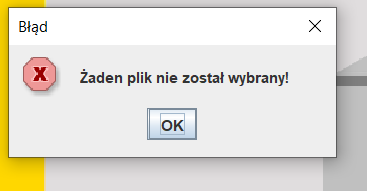
\includegraphics[width=7cm]{blad_5.png}
    \captionof{figure}{}
\end{figure}

\lhead{Reakcje na błędy}

\subsection{Błędy krytyczne}
Błędy krytyczne pojawiają się wtedy, gdy kontynuowanie gry nie jest możliwe.
np. Zostanie usunięty obraz tła (Obrazek 10).

\begin{figure} [hbt!]
    \centering
    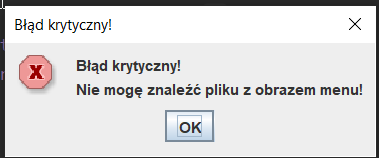
\includegraphics[width=8cm]{krytyczny.png}
    \captionof{figure}{}
\end{figure}

We wszystkich wyżej wymienionych przykładach poza komunikatami pojawia się także dźwięk sygnalizujący błąd.


\section{Prawidłowy sposób uruchomienia programu}
W celu prawidłowego uruchomienia aplikacji wystarczy na nią dwukrotnie nacisnąć, gdyż został został stworzony odpowiedni Manifest. Można także skorzystać z polecania ,,java -jar'', lecz program został napisany w taki sposób, aby wszystkie komunikaty pojawiały się w formie wyskakujących okienek, a nie informacji w konsoli, dlatego sposób ten nie jest to konieczny.
Po wykonaniu jednej z tych operacji wyświetli się Menu, gdzie użytkownik może załączyć plik konfiguracyjny (lub grać z domyślnym), wybrać imiona graczy, zdecydować, czy chce grać z dźwiękiem czy bez, wybrać maksymalną ilość punktów oraz czas rozgrywki (Obrazek 11).

\lhead{Uruchomienie programu}
\begin{figure} [hbt!]
    \centering
    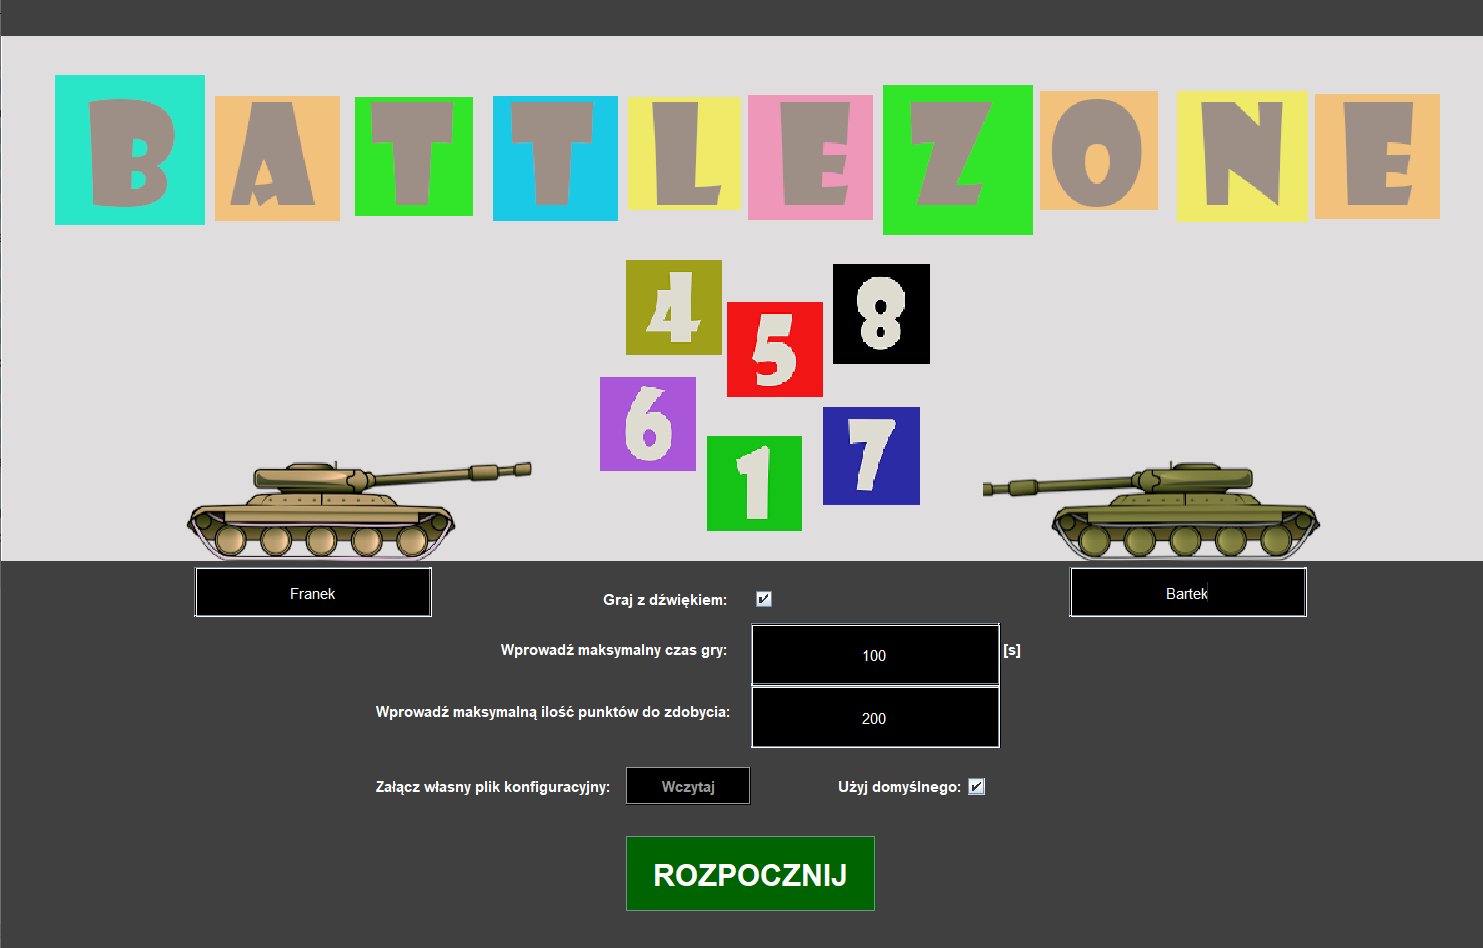
\includegraphics[width=12cm]{menu_panel.png}
    \captionof{figure}{}
\end{figure}


Następnie należy nacisnąć przycisk ,,Rozpocznij'' i rozgrywka się zaczynie. Tak jak założyliśmy w specyfikacji funkcjonalnej użytkownicy mogą poruszać się swoimi czołgami:
\begin{itemize}
\item Prawy użytkownik strzałką w górę i w dół, a lufą strzałkami w prawo i w lewo
\item Lewy użytkownik porusza się klawiszami W - w górę, S - w dół oraz do sterowania lufą służą klawisze A i D 

\newpage Przykład gry znajduje się na rysunku poniżej (Obrazek 12):

\end{itemize}
\begin{figure} [hbt!]
    \centering
    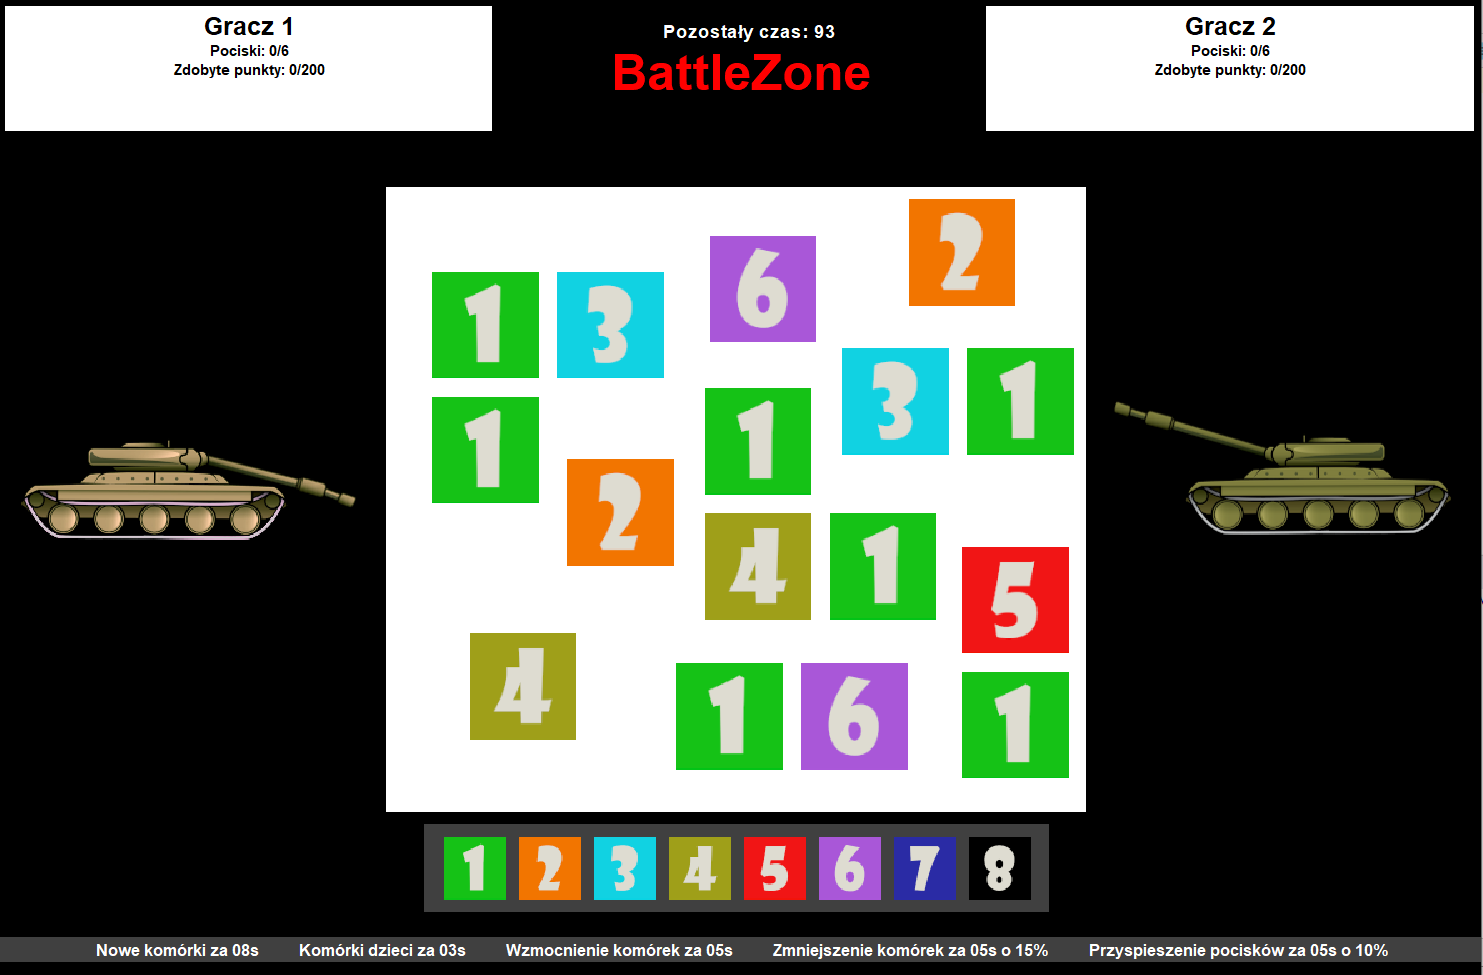
\includegraphics[width=12cm]{rozgrywka.png}
    \captionof{figure}{}
\end{figure}

W prawym i lewym górnym rogu gry znajduje się kolejno imię/nick gracza, jego ilość aktualnie wystrzelonych pocisków oraz zdobytych punktów (Obrazek 13):
\begin{figure} [hbt!]
    \centering
    
\includegraphics[width=7cm]{menu_gracza.png}
    \captionof{figure}{}
\end{figure}
\newline Na samej górze po środku znajduje się czas jaki pozostaje do końca rozgrywki oraz nazwa gry (Obrazek 14):
\begin{figure} [hbt!]
    \centering
    
\includegraphics[width=5cm]{czas_do_konca.png}
    \captionof{figure}{}
\end{figure}
\newpage
Na dole planszy znajduje się dane podane w pliku konfiguracyjnym jak np. czas do powstania nowych komórek, komórek dzieci itd. Fragment poniżej 
(Obrazek 15):
\begin{figure} [hbt!]
    \centering
    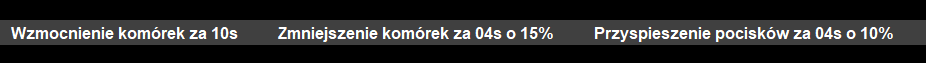
\includegraphics[width=12cm]{pasek.png}
    \captionof{figure}{}
\end{figure}
\newline Istnieje kilka możliwości zakończenia programu, np. Prawy gracz wygrywa poprzez większą ilość punktów (Obrazek 16) albo remis (Obrazek 17):
\begin{figure} [hbt!]
    \centering
    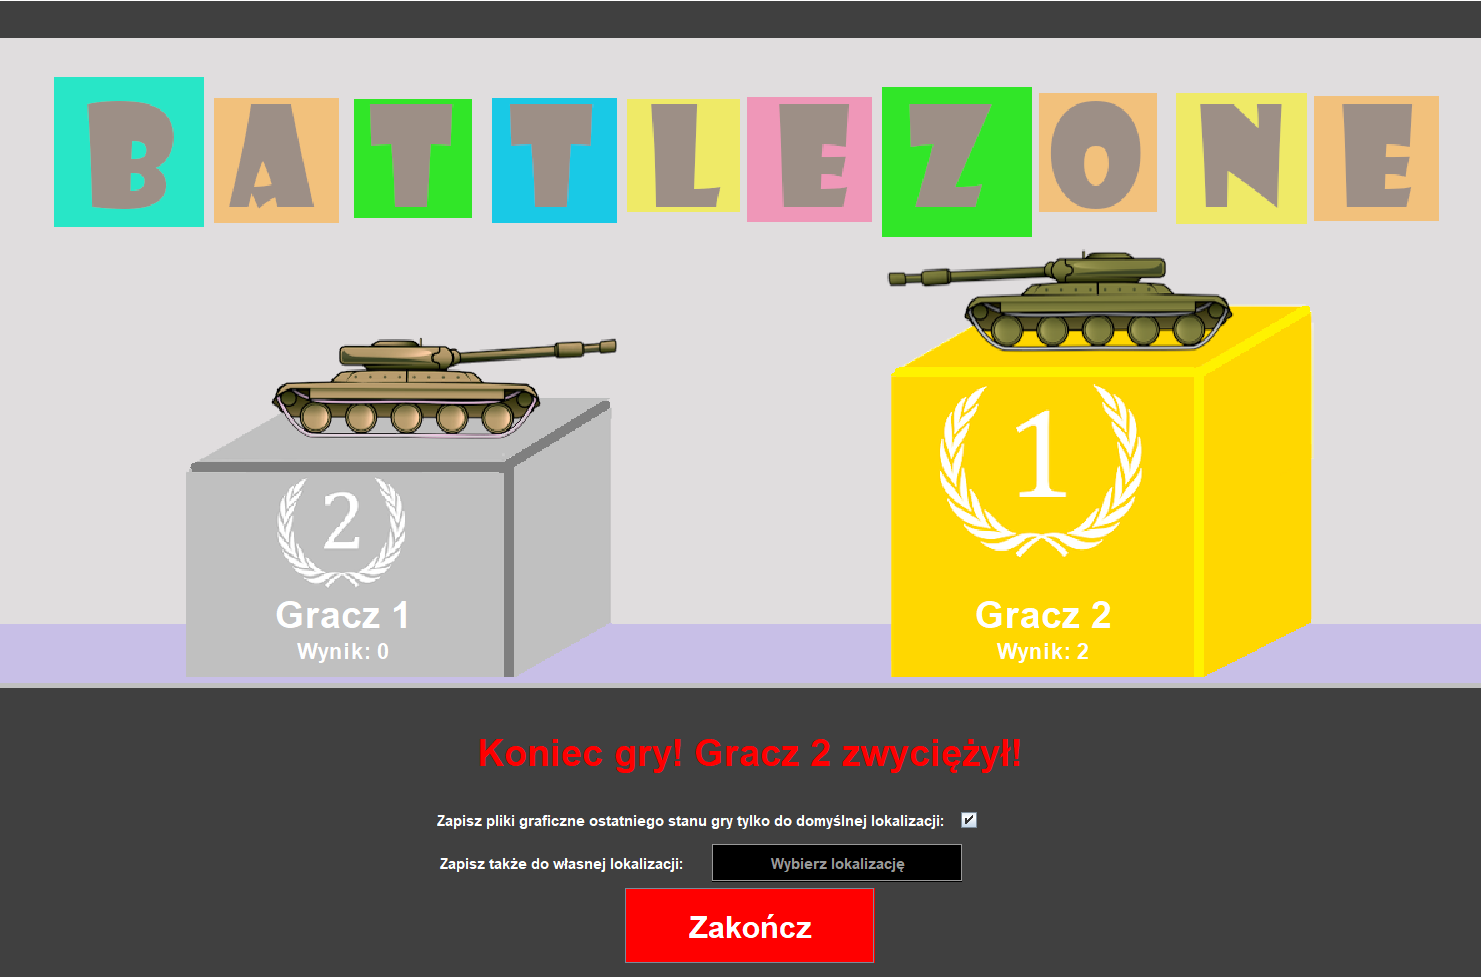
\includegraphics[width=9cm]{koniec_1.png}
    \captionof{figure}{}
\end{figure}
\begin{figure} [hbt!]
    \centering
    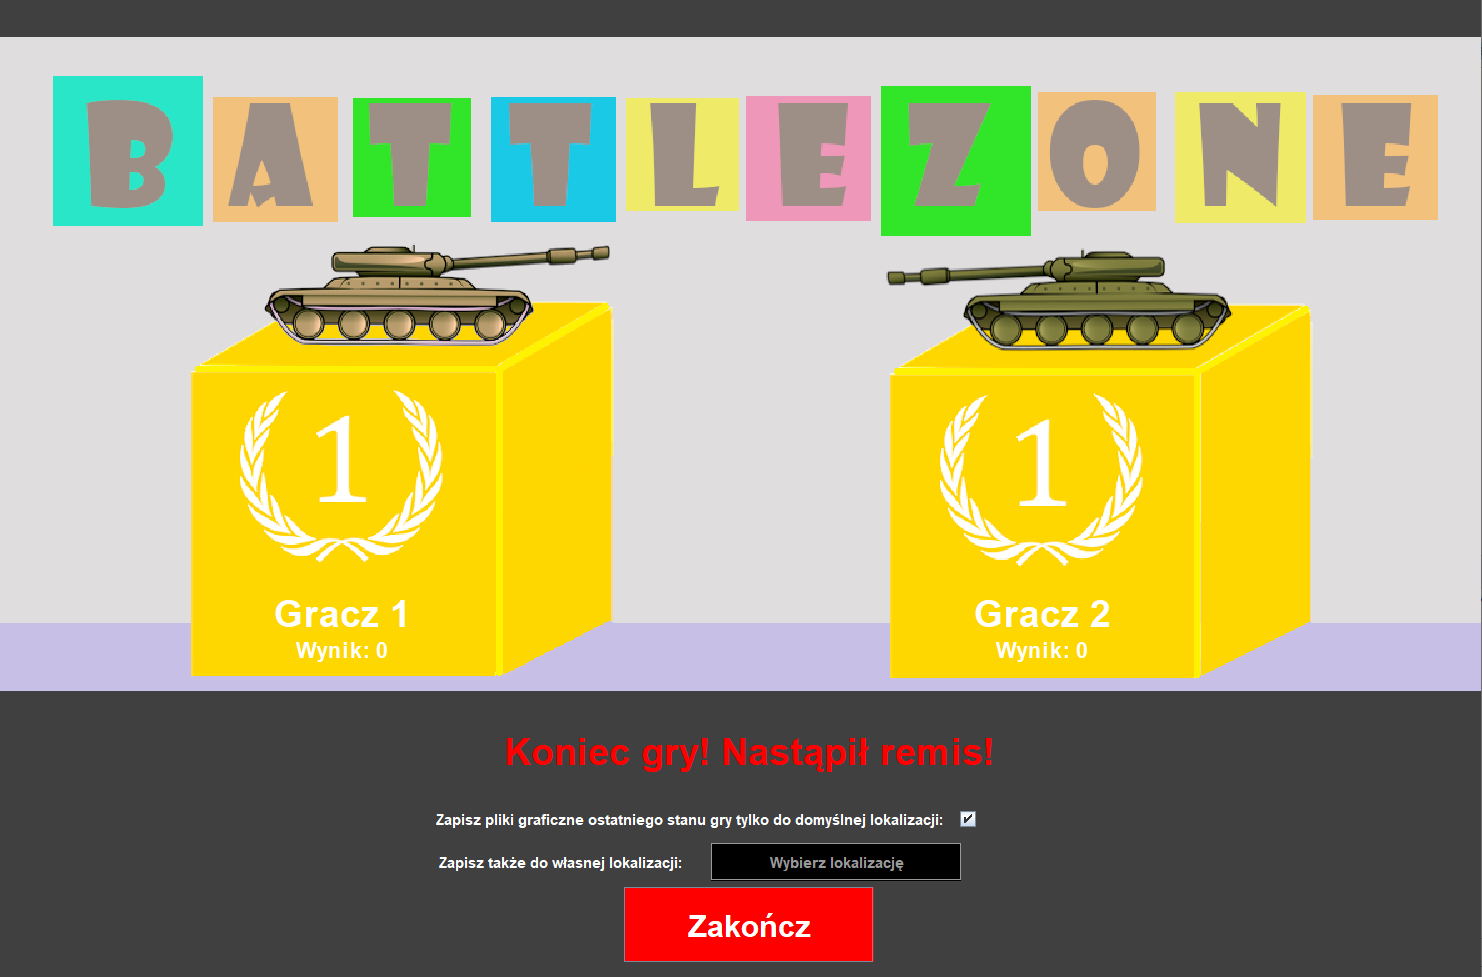
\includegraphics[width=9cm]{koniec_2.png}
    \captionof{figure}{}
\end{figure}

Nad przyciskiem ,,Zakończ'' znajduje się możliwość zapisu planszy do pliku o rozszerzeniu png, w przypadku niewybrania lokalizacji, zdjęcia zostaną zapisane w lokalizacji domyślnej - katalogu, w którym znajduje się aplikacja (Obrazek 18), natomiast w przypadku chęci zapisu do własnej lokalizacji pojawi się okno zapisu (Obrazek 19):
\begin{figure} [hbt!]
    \centering
    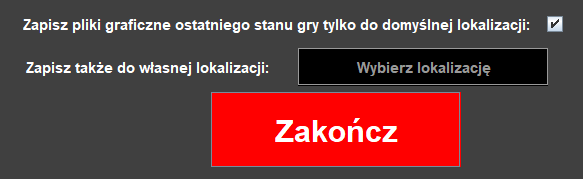
\includegraphics[width=12cm]{zapis_do_pliku.png}
    \captionof{figure}{}
\end{figure}

\begin{figure} [hbt!]
    \centering
    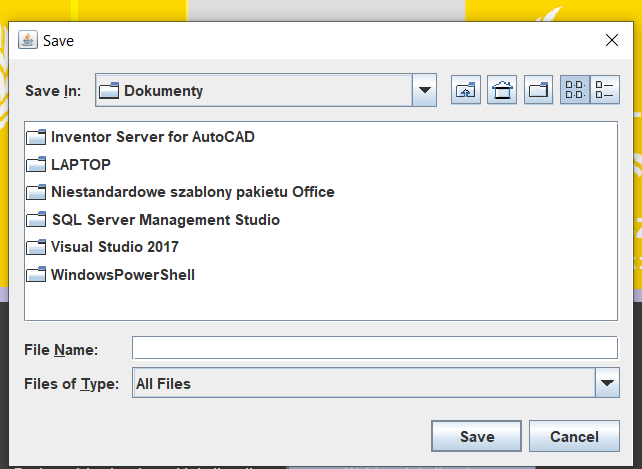
\includegraphics[width=11cm]{zapis.png}
    \captionof{figure}{}
\end{figure}

\lhead{Uruchomienie programu}
Jeżeli użytkownik się pomyli i poda nazwę pliku z rozszerzeniem innym niż png, program sam dostosuje to rozszerzenie.

Efektem wybrania lokalizacji przez użytkownika/skorzystania z lokalizacji domyślnej jest stworzenie dwóch obrazków, jeden z planszą na której znajdują się komórki (Obrazek 20) oraz drugi na którym znajduje się cały końcowy panel gry (Obrazek 21):

\begin{figure}[hbt!]
 \begin{minipage}{5cm}
    \centering
    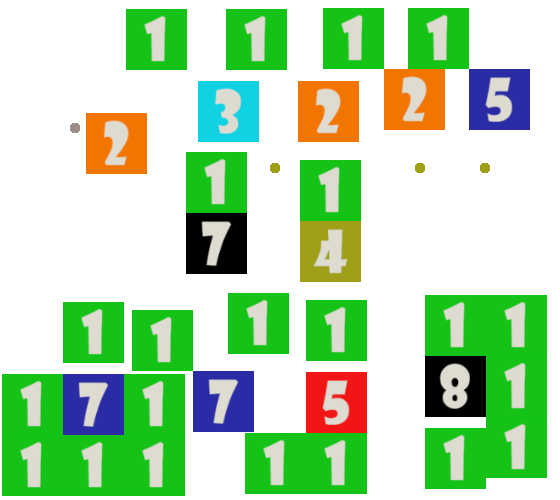
\includegraphics[width=5cm]{koncowa_planszaBoard.png}
    \captionof{figure}{}
 \end{minipage}
 \begin{minipage}{7cm}
    \centering
    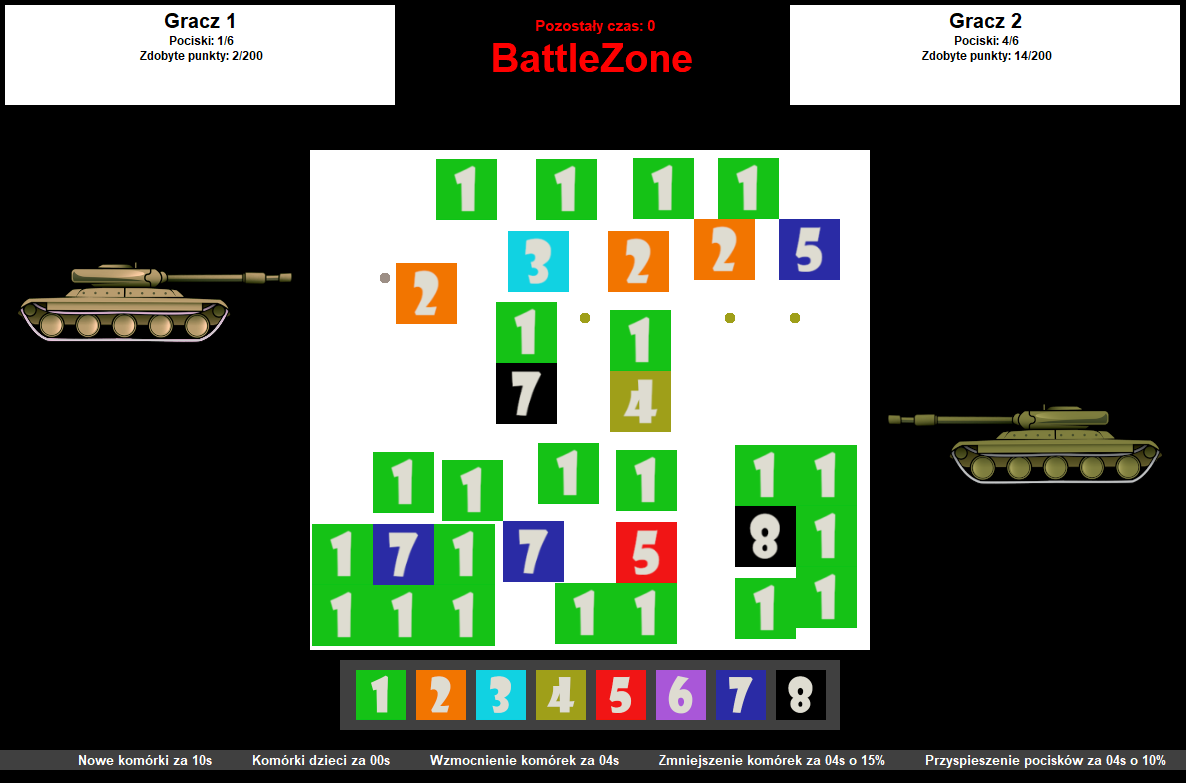
\includegraphics[width=7cm]{koncowa_planszaPanel.png}
    \captionof{figure}{}
 \end{minipage}
\end{figure}


\section{Poprawny format danych w pliku wejściowym}
Wszystkie dane w pliku powinny być zapisane w następujący sposób w pliku z rozszerzeniem txt (Obrazek 22):
\begin{figure} [hbt!]
    \centering
    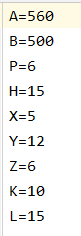
\includegraphics[width=1.5cm]{plik_conf.png}
    \captionof{figure}{}
\end{figure}

\lhead{Plik wejściowy}
W przeciwnym razie program nie pozwoli na rozpoczęcie gry z tym plikiem wejściowym (Obrazek 5). Istnieje możliwość uruchomienia gry z domyślnym plikiem tekstowym. W tym celu należy pozostawić pola tak jak na obrazku poniżej 
(Obrazek 23):
\begin{figure} [hbt!]
    \centering
    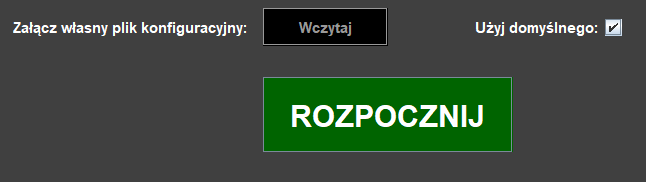
\includegraphics[width=8cm]{wczyt_pliku_conf.png}
    \captionof{figure}{}
\end{figure}

\newpage
Gdy użytkownik będzie chciał załączyć własny plik pojawi się poniższe okno (Obrazek 24):
\begin{figure} [hbt!]
    \centering
    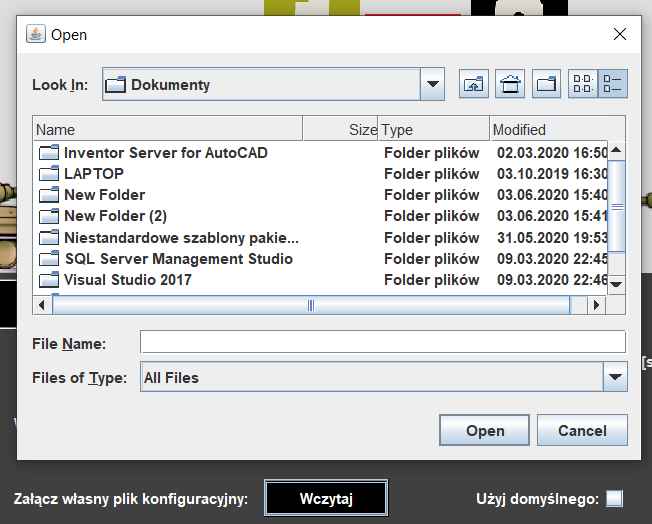
\includegraphics[width=12cm]{wczytanie.png}
    \captionof{figure}{}
\end{figure}

\lhead{Plik wejściowy}

Gdy plik będzie poprawny, a dane będą w odpowiednich zakresach to przycisk zmieni kolor na zielony (Obrazek 25), w przeciwnym razie wyświetli się komunikat o błędzie (Obrazek 9).
\begin{figure} [hbt!]
    \centering
    
\includegraphics[width=10cm]{wczytaj.png}
    \captionof{figure}{}
\end{figure}

\newpage

\section{Wykorzystywane narzędzia oraz podział prac}
\begin{itemize}
    \item Maven:
Narzędzie to okazało się bardzo pomocne. Maven posłużył nam  w automatyzacji budowania aplikacji, wykorzystania zewnętrznych bibliotek oraz uruchamiania testów.

    \item Git:
Repozytorium gita posłużyło nam do pracy równoległej na wielu branchach, testowania nowych rozwiązań i kilkukrotnie do powrotu do wcześniejszych.

    \item Intellij:
Powyższe środowisko bardzo ułatwiło pracę nad kodem. Korzystaliśmy z wielu skrótów klawiszowych, pluginów i innych udogonień tego programu, dzięki czemu praca była szybsza i przyjemniejsza.

    \item Gimp:
Stworzenie grafiki (sprite) czołgu, komórek, tła.

    \item Paint:
Wstępna wizualizacja gry.

    \item Texture Packer GUI:
Pakowanie grafik (sprites) do jednej (spritesheet).

    \item Launch4U:
Przekonwertowanie pliku jar do exe. (Oba te pliki przygotowaliśmy w podkatalogu FINAL\_RELEASE wraz z przykładowymi danymi konfiguracyjnymi).
    \item Bardzo często sięgaliśmy także do dokumentacji Javy ze strony Oracle i szukaliśmy przydatnych rozwiązań.
Wykorzystaliśmy także strony z darmową licencją takie jak: OpenGameArt.org do znalezienia dźwięków do gry oraz favpng.com do znalezienia grafiki czołgu, którą w Gimpie przerobiliśmy na dwa czołgi o różnych ułożeniach lufy.
\end{itemize}
Podział prac:

Bartosz odpowiadał za wczytanie danych z pliku wejściowego, komórki, zapis do pliku.

Franciszek odpowiadał za klasę odpowiedzialną za pociski, panele, graczy oraz grafiki.


Wspólnie opracowaliśmy plan oraz sposób działania naszego programu, stworzyliśmy silnik gry, testy, dobraliśmy dźwięki i kolory do programu, wykonaliśmy sprawozdanie końcowe oraz obie specyfikacje.


Przy następnym projekcie zadbalibyśmy lepiej o częstsze wymienianie się pomysłami oraz konsultowanie wprowadzanych zmian.

\lhead{Narzędzia i podział prac}
\section{Podsumowanie i wnioski}
Różnice programu końcowego, między tym co założyliśmy wynikają z nowych pomysłów i udoskonaleń. Przykładem jest stworzenie nieplanowanej klasy Sounds odpowiadającej za dźwięki w programie. Stworzyliśmy wiele udoskonaleń i uproszczeń wykorzystując GUI, dzięki czemu (subiektywnie) program jest estetyczny, a interfejs prosty do użytku.

Staraliśmy się napisać kod czysty i czytelny, dlatego wielokrotnie go refaktoryzowaliśmy. W rezultacie metody są krótkie, konkretne metody odpowiadają za konkretne funkcjonalności, nazwy zmiennych i metod (a takze treści commitów) są pisane  w języku angielskim zgodnie z ogólnymi konwencjami i ograniczyliśmy ilość powtórzeń. Zrezygnowaliśmy także z pisania komentarzy.

Po za tym duży nacisk położyliśmy na tym, aby program odpowiednio reagował na błędy ze strony użytkownika. Finalna wersja została wielokrotnie przetestowana.
Łącznie w programie zostało napisanych 3259 linijek Javy (według plugina Statistics) (Obrazek 26).
\begin{figure} [hbt!]
    \centering
    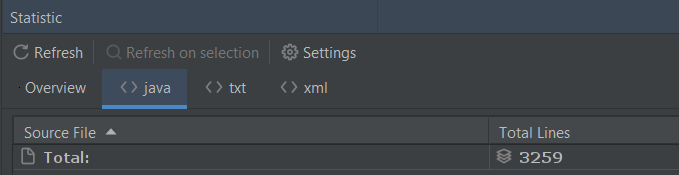
\includegraphics[width=12cm]{statystyki.png}
    \captionof{figure}{}
\end{figure}
Co składa się na 17 klas (w tym 5 testowych).

W programie wyróżniliśmy także 5 dźwięków: wystrzał, koniec gry, tykanie zegara, zestrzelenie komórki oraz dźwięk wyskakującego błędu z Windowsa XP.

Większość czasu, który poświęciliśmy na projekt, poświęciliśmy faktycznie na naukę. Bardzo przydatne okazały się fora, gdzie znajdowaliśmy odpowiedzi na nasze wątpliwości, jak i tutoriale na YouTubie.

Obydwu nam praca nad tym projektem sprawiła przyjemność.
\lhead{Wnioski}
\end{document}
